
\chapter{Presentation of the project}

\section{The goal}

The goal of this project is to create a simulator of Statechart which can be use with UMLDesigner. This simulator should permit to visualize and debug a model of a state machine. Moreover, UMLDesigner is a modeling software for UML model and Statechart, so we could create the model and simulate it on the same tools. The picture \ref{fig:project} represent the aim of this project.

\begin{figure}[h]
  \centering
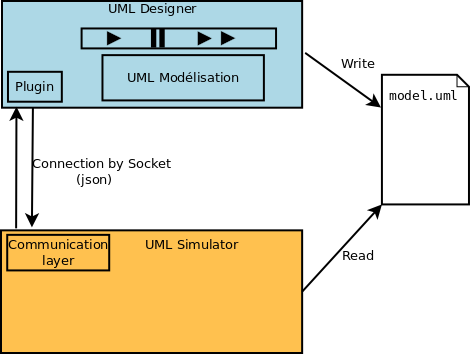
\includegraphics[width=\textwidth]{project}  
  \caption{Description of the project}
  \label{fig:project}
\end{figure}


\section{Tools at the disposal}

At the begin of this project, some of the tools, which were needed, existed. In fact, ULMDesigner is a UML modeling tool develop by \textit{Obeo}. However, it didn't exist yet a simulator for Statechart adapted for UMLDesigner. On the chapter \ref{chap:UMLDesigner}, the running of UMLDesigner will be discuss.~\\

Then, Mr Ciprian Theodorov, one of my professor, has developed a simulator for Statechart. This simulator needed to be improved, but it composed a good beginning for this project. 



%%% Local Variables: 
%%% mode: latex
%%% TeX-master: "../rapport_de_base"
%%% End: 
